% Options for packages loaded elsewhere
\PassOptionsToPackage{unicode}{hyperref}
\PassOptionsToPackage{hyphens}{url}
%
\documentclass[
  12pt,
]{article}
\usepackage{amsmath,amssymb}
\usepackage{iftex}
\ifPDFTeX
  \usepackage[T1]{fontenc}
  \usepackage[utf8]{inputenc}
  \usepackage{textcomp} % provide euro and other symbols
\else % if luatex or xetex
  \usepackage{unicode-math} % this also loads fontspec
  \defaultfontfeatures{Scale=MatchLowercase}
  \defaultfontfeatures[\rmfamily]{Ligatures=TeX,Scale=1}
\fi
\usepackage{lmodern}
\ifPDFTeX\else
  % xetex/luatex font selection
\fi
% Use upquote if available, for straight quotes in verbatim environments
\IfFileExists{upquote.sty}{\usepackage{upquote}}{}
\IfFileExists{microtype.sty}{% use microtype if available
  \usepackage[]{microtype}
  \UseMicrotypeSet[protrusion]{basicmath} % disable protrusion for tt fonts
}{}
\makeatletter
\@ifundefined{KOMAClassName}{% if non-KOMA class
  \IfFileExists{parskip.sty}{%
    \usepackage{parskip}
  }{% else
    \setlength{\parindent}{0pt}
    \setlength{\parskip}{6pt plus 2pt minus 1pt}}
}{% if KOMA class
  \KOMAoptions{parskip=half}}
\makeatother
\usepackage{xcolor}
\usepackage[margin=2.5cm]{geometry}
\usepackage{longtable,booktabs,array}
\usepackage{calc} % for calculating minipage widths
% Correct order of tables after \paragraph or \subparagraph
\usepackage{etoolbox}
\makeatletter
\patchcmd\longtable{\par}{\if@noskipsec\mbox{}\fi\par}{}{}
\makeatother
% Allow footnotes in longtable head/foot
\IfFileExists{footnotehyper.sty}{\usepackage{footnotehyper}}{\usepackage{footnote}}
\makesavenoteenv{longtable}
\usepackage{graphicx}
\makeatletter
\newsavebox\pandoc@box
\newcommand*\pandocbounded[1]{% scales image to fit in text height/width
  \sbox\pandoc@box{#1}%
  \Gscale@div\@tempa{\textheight}{\dimexpr\ht\pandoc@box+\dp\pandoc@box\relax}%
  \Gscale@div\@tempb{\linewidth}{\wd\pandoc@box}%
  \ifdim\@tempb\p@<\@tempa\p@\let\@tempa\@tempb\fi% select the smaller of both
  \ifdim\@tempa\p@<\p@\scalebox{\@tempa}{\usebox\pandoc@box}%
  \else\usebox{\pandoc@box}%
  \fi%
}
% Set default figure placement to htbp
\def\fps@figure{htbp}
\makeatother
\setlength{\emergencystretch}{3em} % prevent overfull lines
\providecommand{\tightlist}{%
  \setlength{\itemsep}{0pt}\setlength{\parskip}{0pt}}
\setcounter{secnumdepth}{-\maxdimen} % remove section numbering
\usepackage{fancyhdr}
\pagestyle{fancy}
\fancyhf{} % clear header and footer

% Header
\fancyhead[L]{Nino Gerber}                                % Left: Your name
\fancyhead[C]{Poisson Regression Analysis}                % Center: Report title (short version)
\fancyhead[R]{\today}                                     % Right: Current date

% Footer
\fancyfoot[C]{\thepage}                                   % Center: Page number
\usepackage{booktabs}
\usepackage{longtable}
\usepackage{array}
\usepackage{multirow}
\usepackage{wrapfig}
\usepackage{float}
\usepackage{colortbl}
\usepackage{pdflscape}
\usepackage{tabu}
\usepackage{threeparttable}
\usepackage{threeparttablex}
\usepackage[normalem]{ulem}
\usepackage{makecell}
\usepackage{xcolor}
\usepackage{bookmark}
\IfFileExists{xurl.sty}{\usepackage{xurl}}{} % add URL line breaks if available
\urlstyle{same}
\hypersetup{
  pdftitle={Poisson Regression Analysis of Apprentice Migration},
  pdfauthor={Nino Gerber},
  hidelinks,
  pdfcreator={LaTeX via pandoc}}

\title{Poisson Regression Analysis of Apprentice Migration}
\author{Nino Gerber}
\date{2025-05-17}

\begin{document}
\maketitle

\section{Introduction}\label{introduction}

This report investigates factors influencing the number of apprentices
migrating from various regions to Edinburgh. The response variable is
the \textbf{count of apprentices}, and the predictors are
\textbf{distance from Edinburgh}, \textbf{population of the region},
\textbf{degree of urbanization}, and \textbf{direction from Edinburgh}.
The scientific question is: \emph{Which geographical and demographic
factors significantly predict the number of apprentices migrating to
Edinburgh between 1775 and 1799, and how do these relationships vary
across regions?}

The dataset records the number of apprentices moving to Edinburgh
between 1775 and 1799 from other Scottish counties. During this period,
Edinburgh was a significant center for trade and education, attracting
young individuals looking for apprenticeship opportunities.
Understanding the patterns of apprentice migration during this time
provides valuable insights into the socio-economic factors influencing
labor mobility in the 18th-century in Scotland. (Lovett \& Flowerdew,
1989).

\section{Descriptive Statistics}\label{descriptive-statistics}

This section provides an overview of the key variables in the dataset.
The dataset used in this analysis was obtained from
\url{http://users.stat.ufl.edu/~winner/data/apprentice.txt}. It contains
the following variables:

\begin{itemize}
\tightlist
\item
  \texttt{region}: Region name
\item
  \texttt{apprentices}: Number of apprentices (response variable)
\item
  \texttt{distance}: Distance from Edinburgh (in miles)
\item
  \texttt{population}: Population of the region (in thousands)
\item
  \texttt{urban}: Urbanization score (numeric)
\item
  \texttt{direction}: Cardinal direction from Edinburgh (coded as a
  factor: 1=North, 2=West, 3=South).
\end{itemize}

\textbf{Numerical Variables:} Table 1 presents the minimum, median,
mean, and maximum values for four continuous variables:

\begin{longtable}[]{@{}lrrrr@{}}
\caption{Clean Summary Statistics of the Main Variables}\tabularnewline
\toprule\noalign{}
Variable & Min & Median & Mean & Max \\
\midrule\noalign{}
\endfirsthead
\toprule\noalign{}
Variable & Min & Median & Mean & Max \\
\midrule\noalign{}
\endhead
\bottomrule\noalign{}
\endlastfoot
Distance & 21.0 & 92.0 & 131.8 & 491.0 \\
Apprentices & 0.0 & 3.0 & 14.2 & 225.0 \\
Population & 5.0 & 30.0 & 46.6 & 147.0 \\
Urbanization & 7.7 & 27.3 & 28.6 & 69.9 \\
\end{longtable}

The figures in table 1 show that while most counties contributed few
apprentices (median = 3), some---such as Midlothian---had significantly
higher counts, driving the mean up to 14.2. Similarly, distances vary
widely, with some regions more than 400 miles from Edinburgh.

\textbf{Categorical Variable, Direction: } The dataset also categorizes
each county into one of three cardinal directions relative to Edinburgh:
North, West, and South. The majority of counties are located in the
North (49\%), followed by the South (27\%) and West (24\%). There are 33
different counties in the data set and therefore 33 records.

\subsubsection{Counties with the Most and Fewest
Apprentices}\label{counties-with-the-most-and-fewest-apprentices}

To better understand spatial disparities in apprentice migration, table
2 highlights the counties with the highest number of apprentices

\begin{longtable}[]{@{}lrrrrl@{}}
\caption{Top 5 Counties with the Most Apprentices}\tabularnewline
\toprule\noalign{}
region & apprentices & distance & population & urban & direction \\
\midrule\noalign{}
\endfirsthead
\toprule\noalign{}
region & apprentices & distance & population & urban & direction \\
\midrule\noalign{}
\endhead
\bottomrule\noalign{}
\endlastfoot
Midlothian & 225 & 21 & 56 & 18.8 & South \\
East Lothian & 44 & 33 & 30 & 43.4 & South \\
Fife & 41 & 36 & 94 & 41.3 & North \\
Perth & 26 & 78 & 126 & 14.4 & North \\
Lanark & 23 & 54 & 147 & 68.1 & West \\
\end{longtable}

These top counties are either located close to Edinburgh (e.g.,
Midlothian, East Lothian) or have high population and urbanization
scores, suggesting accessibility and economic opportunity may have
facilitated apprentice movement

By investigating the dataset, we observe that 7 out of 33 Scottish
counties report zero apprentices. This is likely to impact the modeling
later on and should be taken into account. These counties tend to have
low population sizes (ranging from 8 to 29 thousand) and high distances
from Edinburgh (between 79 and 366 miles). Their urbanization scores
vary from 9 to 43.6. This suggests that accessibility---captured by
distance---as well as population size and urbanization, may influence
apprentice migration. Notably, the counties with zero apprentices are
evenly distributed across the North, South, and West.

\section{Exploratory Data Analysis}\label{exploratory-data-analysis}

This section provides an overview of the data using correlation
analysis, histograms, and scatterplots to guide model specification.

\subsection{Correlation Matrix and Distribution
Overview}\label{correlation-matrix-and-distribution-overview}

To understand both the individual variables and their pairwise
relationships, we use a correlation matrix with embedded histograms and
scatterplots. This helps guide model choice and transformations.

\begin{figure}
\centering
\pandocbounded{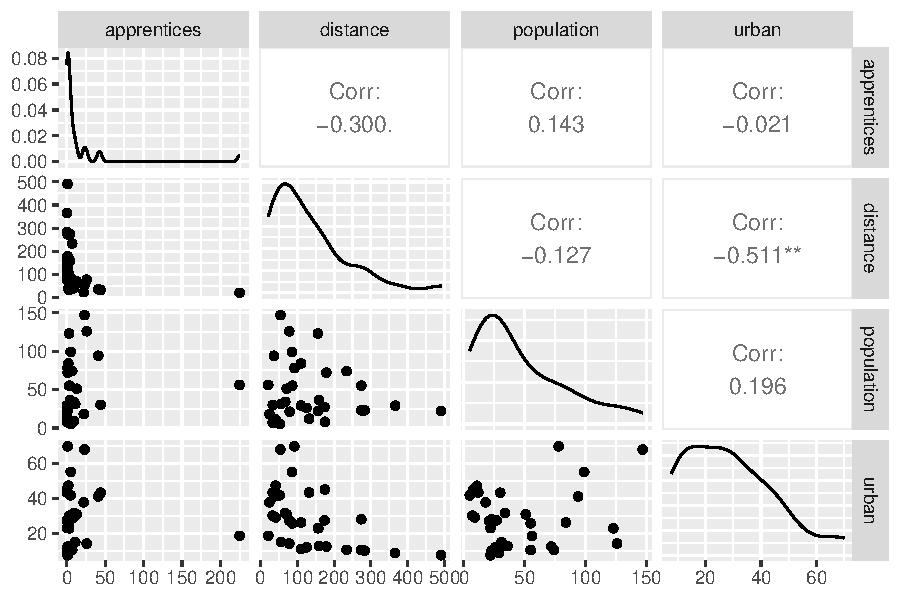
\includegraphics[keepaspectratio]{poisson_apprentice_report_files/figure-latex/bivariate-1.pdf}}
\caption{Correlation Matrix and Distribution Plots}
\end{figure}

\textbf{Apprentices (Response Variable): } Apprenticeship counts are
heavily right-skewed, with most regions sending few apprentices and one
clear outlier (Midlothian).

\textbf{Distance (Predictor):} Shows a moderate negative correlation
with apprentices (r = --0.30), making it a key predictor. Distances
range from 21 to 491 miles, with most counties located within 50--150
miles of Edinburgh.

\textbf{Population (Predictor):} The distribution is right-skewed, with
most counties having fewer than 50,000 residents. It shows a weak
positive association with apprentice counts (r = 0.14), suggesting some
influence.

\textbf{Urbanization (Predictor):} Also right-skewed, with no meaningful
linear correlation with apprentices (r = --0.02). However, non-linear or
regional effects may be present.

\textbf{Distance and Urbanization:} Strongly negatively correlated (r =
--0.51), suggesting potential multicollinearity if both variables are
included in the model

The histograms help identify skewed distributions, potential outliers
(e.g., Midlothian), and the overall data spread---informing model choice
and interpretation. The matrix confirms distance as the most informative
predictor and highlights overlap with urbanization, warranting caution
in joint interpretation.

\subsection{Bivariate Analysis}\label{bivariate-analysis}

To examine the influence of direction and the effect of
log-transformations on the predictors, we present the following
scatterplots.

\begin{figure}
\centering
\pandocbounded{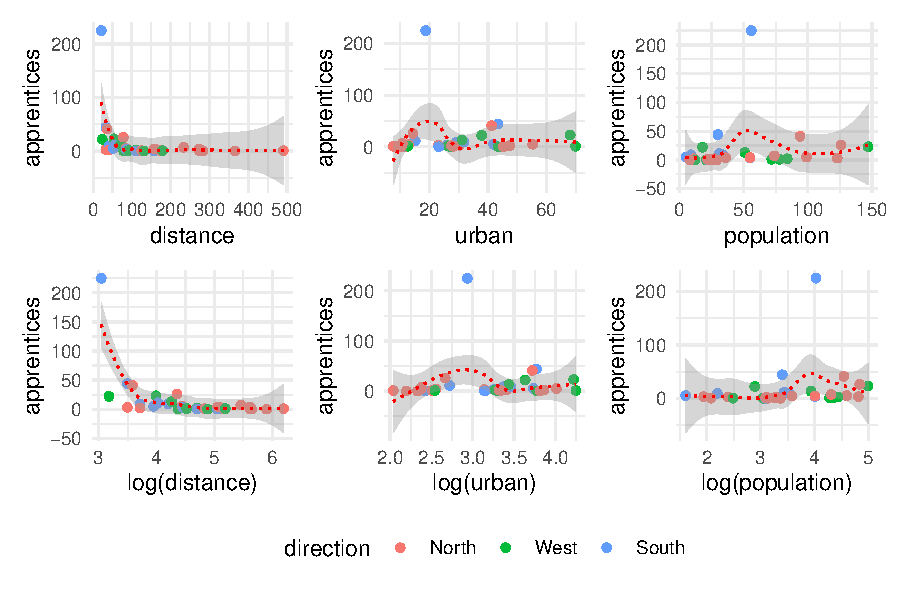
\includegraphics[keepaspectratio]{poisson_apprentice_report_files/figure-latex/univariate2-1.pdf}}
\caption{Apprentices by Region and Demographic Factors}
\end{figure}

The lower row of scatterplots presents the same relationships using
log-transformed predictors, which help linearize skewed distributions
and stabilize variance. The effect of distance becomes more regular,
reinforcing its role as a strong negative predictor. Urbanization still
shows no consistent pattern, though subtle regional differences persist.
For population, the log transformation slightly clarifies the weak
positive trend, but regional variability remains high.

These refined plots illustrate the utility of log transformations in
preparing variables for modeling, and further support the inclusion of
interaction terms between direction and distance or population.

\section{Poisson Regression Model}\label{poisson-regression-model}

\subsection{Model Definitions}\label{model-definitions}

Let \(Y_i\) be the number of apprentices in region \(i\), assumed to
follow a Poisson distribution:

\[
Y_i \sim \text{Poisson}(\lambda_i), \quad \log(\lambda_i) = \eta_i
\]

Model fitting is performed via \textbf{maximum likelihood estimation}

We build several models to compare the influence of the predictors in
the dataset. The linear predictors \(\eta_i\) for the six Poisson models
are defined as:

\begin{align*}
\textbf{Model 0:} \quad 
\eta_i &= \beta_0 + \beta_1 \cdot d_i + \beta_2 \cdot p_i + \beta_3 \cdot \text{Dir}_i \\
\\
\textbf{Model 1:} \quad 
\eta_i &= \beta_0 + \beta_1 \cdot d_i + \beta_2 \cdot p_i + \beta_3 \cdot \text{Dir}_i + \beta_4 \cdot (p_i \times \text{Dir}_i) \\
\\
\textbf{Model 2:} \quad 
\eta_i &= \beta_0 + \beta_1 \cdot d_i + \beta_2 \cdot \text{Dir}_i + \beta_3 \cdot (d_i \times \text{Dir}_i) + \beta_4 \cdot p_i \\
\\
\textbf{Model 3:} \quad 
\eta_i &= \beta_0 + \beta_1 \cdot \log(d_i) + \beta_2 \cdot \text{Dir}_i + \beta_3 \cdot (\log(d_i) \times \text{Dir}_i) \\
       &\quad + \beta_4 \cdot \log(p_i) + \beta_5 \cdot u_i \\
\\
\textbf{Model 4:} \quad 
\eta_i &= \beta_0 + \beta_1 \cdot \log(d_i) + \beta_2 \cdot \text{Dir}_i + \beta_3 \cdot (\log(d_i) \times \text{Dir}_i) + \beta_4 \cdot \log(p_i) \\
\\
\textbf{Model 5:} \quad 
\eta_i &= \beta_0 + \beta_1 \cdot \log(d_i) + \beta_2 \cdot \log(p_i)
\end{align*}

\[
\textbf{Zero-Inflated Poisson Model:} \quad 
Y_i \sim \begin{cases}
0 & \text{with probability } \pi_i                                       \\
\text{Poisson}(\eta_i) & \text{with probability } 1 - \pi_i         
\end{cases}
\quad
\]

\[
\text{with }\eta_i = \beta_0 + \beta_1 \cdot d_i + \beta_2 \cdot \text{Dir}_i + \beta_3 \cdot (d_i \times \text{Dir}_i) + \beta_4 \cdot p_i
\]

\[ \text{and a constant zero-inflation term modeled by a logistic function: logit}(\pi_i) =\gamma_0\]

\textbf{Abbreviation Key:}\\
\texttt{Int} = Intercept, \texttt{d} = distance, \texttt{p} =
population, \texttt{dW} = directionWest, \texttt{dS} = directionSouth,
\texttt{p:dW} = population × directionWest, \texttt{p:dS} = population ×
directionSouth, \texttt{d:dW} = distance × directionWest, \texttt{d:dS}
= distance × directionSouth, \texttt{log(d)} = log(distance),
\texttt{log(p)} = log(population), \texttt{log(d):dW} = log(distance) ×
directionWest,\texttt{log(d):dS} = log(distance) × directionSouth.

Each model adds complexity in a controlled way to assess trade-offs
between interpretability and fit quality (via AIC/log-likelihood). The
goal is to identify the most parsimonious model that captures relevant
spatial and demographic effects.

\begin{itemize}
\tightlist
\item
  Model 0--2 include linear predictors and interaction terms to capture
  spatial heterogeneity.
\item
  Model 3--5 introduce logarithmic transformations to reduce skewness
  and potentially improve fit.
\item
  The \textbf{ZIP model} is used to account for \textbf{excess zeros},
  which may arise in rural or low-population regions with no apprentices
  at all.
\end{itemize}

\subsection{Model Fitting}\label{model-fitting}

The model is fitted via \textbf{Maximum Likelihood Estimation (MLE)},
maximizing the Poisson likelihood:

\[
\mathcal{L}(\boldsymbol{\beta}) = \prod_{i=1}^n \frac{\lambda_i^{y_i} e^{-\lambda_i}}{y_i!}
\]

\begin{table}[!h]
\centering
\caption{\label{tab:model-summary-table_2}Table: Summary of Model Fit Statistics}
\centering
\begin{tabular}[t]{>{}lrrr}
\toprule
Model & AIC & LogLik & df\\
\midrule
\textbf{\cellcolor{gray!10}{Model 0}} & \cellcolor{gray!10}{442.7} & \cellcolor{gray!10}{-216.3} & \cellcolor{gray!10}{28}\\
\textbf{Model 1} & 323.3 & -154.7 & 26\\
\textbf{\cellcolor{gray!10}{Model 2}} & \cellcolor{gray!10}{212.7} & \cellcolor{gray!10}{-99.3} & \cellcolor{gray!10}{26}\\
\textbf{Model 3} & 162.2 & -73.1 & 25\\
\textbf{\cellcolor{gray!10}{Model 4}} & \cellcolor{gray!10}{162.8} & \cellcolor{gray!10}{-74.4} & \cellcolor{gray!10}{26}\\
\addlinespace
\textbf{Model 5} & 259.6 & -126.8 & 30\\
\textbf{\cellcolor{gray!10}{ZIP Model}} & \cellcolor{gray!10}{214.7} & \cellcolor{gray!10}{-99.3} & \cellcolor{gray!10}{NA}\\
\bottomrule
\end{tabular}
\end{table}

\subsubsection{Model Assumptions}\label{model-assumptions}

Poisson regression relies on the following key assumptions (Dobson \&
Barnett, 2018; Agresti, 2007):

\begin{itemize}
\tightlist
\item
  The response variable is a count (non-negative integers).
\item
  Observations are independent.
\item
  The log of the expected count is a linear function of the predictors.
\item
  The conditional mean equals the conditional variance (equidispersion).
\end{itemize}

We test these assumptions using diagnostic plots and overdispersion
analysis (see below).

\section{Model Assessment}\label{model-assessment}

To compare models, we use:

\paragraph{1. Akaike Information Criterion
(AIC)}\label{akaike-information-criterion-aic}

\[
\text{AIC} = 2k - 2 \log \hat{\mathcal{L}}
\]

where: - \(k\) is the number of parameters (degrees of freedom), -
\(\hat{\mathcal{L}}\) is the maximized likelihood.

Lower AIC values indicate better model performance while penalizing
complexity.

\paragraph{2. Degrees of Freedom (df)}\label{degrees-of-freedom-df}

\[
\text{df} = n - k
\]

where: - \(n\) is the number of observations, - \(k\) is the number of
estimated parameters.

Table 3 provides a summary of the fitted models. Among all models
tested, Model 3---which includes log-transformed distance, direction,
urbanization, and their interactions---had the lowest AIC (162.18) and
residual deviance, indicating the best overall fit. Simpler models, such
as Model 0 (AIC = 442.7), performed significantly worse. Model 2, which
includes a distance × direction interaction, showed improved fit (AIC =
212.7) but was still outperformed by the log-transformed models. The
Zero-Inflated Poisson (ZIP) model achieved a similar fit to Model 2 (AIC
= 214.7) but introduced additional complexity by modeling excess zeros.

Although the dataset contains many zeros, a Vuong test comparing the
standard Poisson model to a Zero-Inflated Poisson (ZIP) model found no
significant improvement (z = 0.91, p = 0.18). AIC- and BIC-corrected
statistics strongly favored the standard model. This suggests that the
zeros are well explained by existing covariates, and modeling zero
inflation adds unnecessary complexity.

\begin{figure}
\centering
\pandocbounded{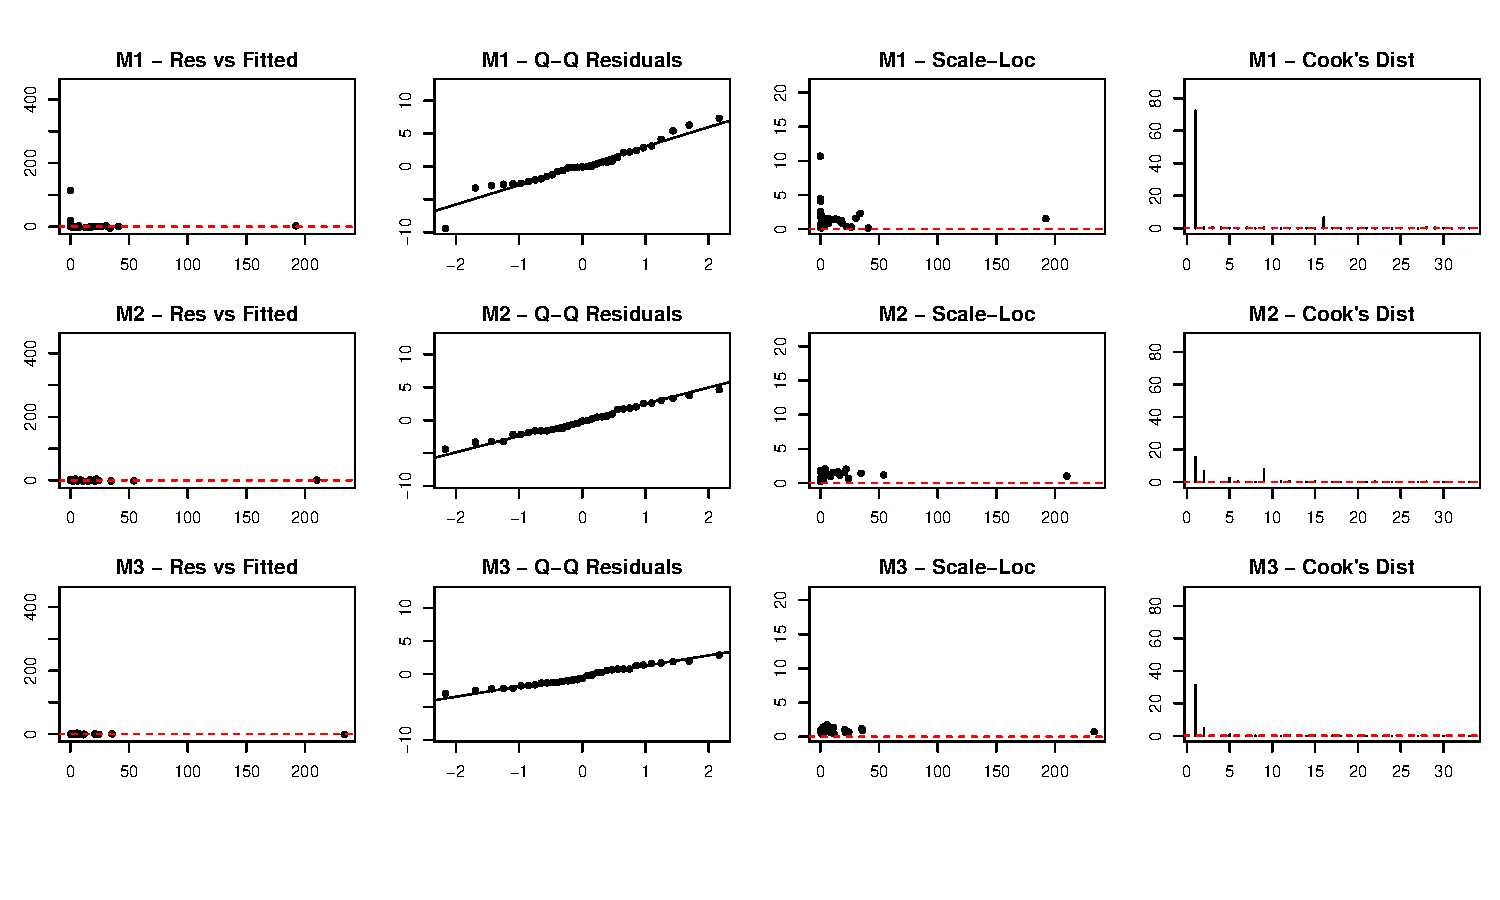
\includegraphics[keepaspectratio]{poisson_apprentice_report_files/figure-latex/model-diagnostics3-1.pdf}}
\caption{Diagnostic plots for Models M3 to M5}
\end{figure}

The residual diagnostic plots for the best Models (AIC), which are model
1--3 (shown in Figure X) include:

\begin{itemize}
\item
  Residuals vs Fitted: to assess non-linearity
\item
  Q-Q Plots: to assess normality of residuals (not assumed in Poisson
  but helps diagnose outliers)
\item
  Scale-Location: to examine homoscedasticity
\item
  Cook's Distance: to identify influential observations
\end{itemize}

Model 1 shows wider spread in residuals, some curvature in the residual
vs fitted plot, and a few high-leverage points (Cook's distance). Model
2 improves upon this, with more linear residual patterns and lower
influence points. Model 3 shows the best residual behavior---residuals
are tightly clustered, with minimal deviation from linearity and no
apparent outliers or influential observations.

\subsection{Overdispersion Analysis}\label{overdispersion-analysis}

A dispersion value close to 1 indicates that the Poisson assumption
(mean ≈ variance) holds. Values substantially greater than 1 suggest
\textbf{overdispersion}, meaning the model underestimates variability in
the data.

The computed dispersion statistics are:

\textbf{Dispersion values} --- Model 0: 7200.29, Model 1: 532.19, Model
2: 4.64, \textbf{Model 3: 1.85}, Model 4: 1.93, Model 5: 8.45, ZIP
Model: 4.81

\subsubsection{Interpretation}\label{interpretation}

\begin{itemize}
\tightlist
\item
  \textbf{Model 0} and \textbf{Model 1} suffer from extreme
  overdispersion, confirming they are inadequate for modeling this data.
\item
  \textbf{Model 2} shows considerable improvement, but a dispersion of
  4.64 still indicates a poor fit.
\item
  \textbf{Models 3 and 4} yield dispersion values close to 2, suggesting
  that these models manage variability relatively well and are more
  appropriate for inference.
\item
  \textbf{Model 5} shows renewed overdispersion (8.45), suggesting that
  its added complexity may not translate into improved fit.
\item
  The \textbf{ZIP model}, despite explicitly modeling excess zeros,
  still shows overdispersion (4.81) and, did not outperform the standard
  Poisson model.
\end{itemize}

\subsubsection{Conclusion}\label{conclusion}

\textbf{Model 3} provides the best balance between goodness of fit and
parsimony. It substantially reduces overdispersion while maintaining
interpretability and a strong AIC performance. This reinforces the
conclusion that the standard Poisson model, with appropriate
transformations and interactions, is sufficient and preferable to more
complex or zero-inflated alternatives. The dispearsion analyse confirms
the choice of poisson regression and dicard the idea of using a
different model like a quasi-poisson model or a negative binomial.

\section{Final Model}\label{final-model}

\subsection{Final Model Specification}\label{final-model-specification}

The final Poisson regression model with a log-link function is given by:

\[
\begin{aligned}
\hat{y}_i = \exp\Big(& 
81 
+ 0.28 \cdot \log(d_i) 
+ 34.76 \cdot \text{dir}_{\text{West},i} \\
& + 198.90 \cdot \text{dir}_{\text{South},i} 
+ 2.46 \cdot \log(\text{pop}_i) 
+ 0.99 \cdot u_i \\
& + 0.39 \cdot \log(d_i) \cdot \text{dir}_{\text{West},i} 
+ 0.29 \cdot \log(d_i) \cdot \text{dir}_{\text{South},i} 
\Big)
\end{aligned}
\]

Where: - log(dᵢ): log-transformed distance from Edinburgh - dirWestᵢ,
dirSouthᵢ: dummy variables for direction (North is baseline) -
log(popᵢ)`: log-transformed regional population - uᵢ: urbanization score
- Interaction terms account for varying distance effects across
directions

\begin{figure}
\centering
\pandocbounded{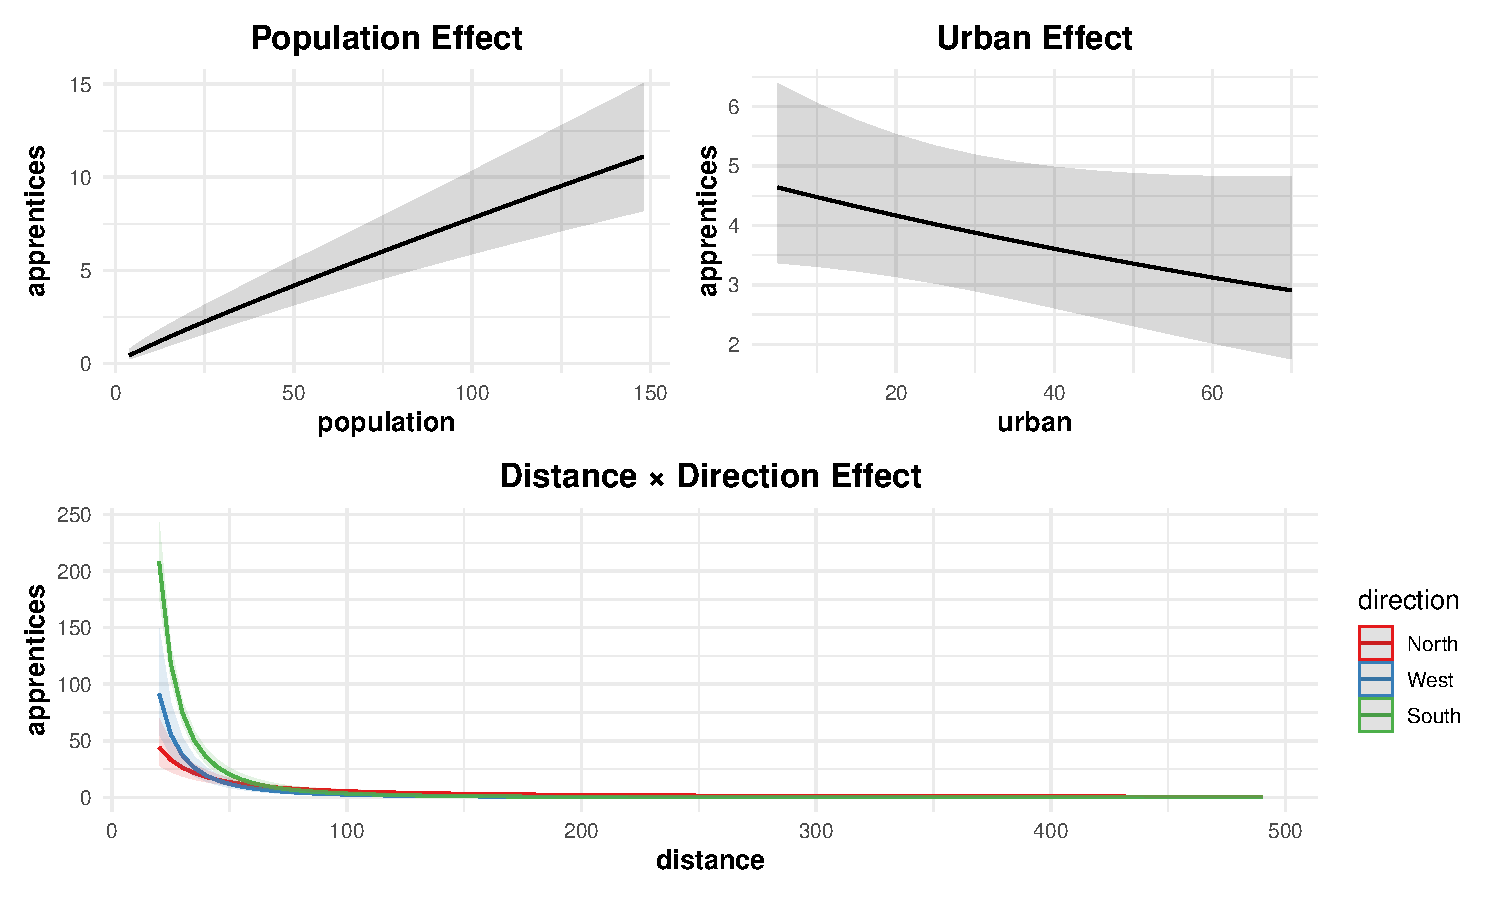
\includegraphics[keepaspectratio]{poisson_apprentice_report_files/figure-latex/combined-effects-1.pdf}}
\caption{Marginal effects of population, urbanization, and distance on
apprentice counts}
\end{figure}

\begin{itemize}
\item
  Population: As county population increases, the number of apprentices
  rises significantly, showing a strong positive effect.
\item
  Urbanization: More urbanized counties send slightly fewer apprentices,
  suggesting urban areas may offer local alternatives.
\item
  Distance × Direction: Apprentice counts drop sharply with increasing
  distance, especially in the South. At equal distances, southern
  counties send more apprentices than western or northern ones.
\end{itemize}

This highlights population size as the main driver, with distance and
geography shaping access

\section{Conclusion}\label{conclusion-1}

This report explored the geographic and demographic factors influencing
apprentice migration to Edinburgh between 1775 and 1799, using Poisson
regression modeling. After evaluating several model specifications,
Model 3, which includes log-transformed distance and population,
urbanization, and interaction terms with direction, emerged as the
best-fitting and most interpretable model.

Key findings include:

\begin{itemize}
\item
  Population size is the strongest positive driver of apprentice counts.
\item
  Urbanization shows a modest negative association, suggesting urban
  regions may offer local opportunities that reduce outward migration.
\item
  Distance significantly decreases apprentice counts, with the effect
  varying by region---southern counties send more apprentices than
  northern or western counties at comparable distances.
\end{itemize}

Despite the presence of many zeros in the data, zero-inflated models did
not provide a better fit, confirming that a well-specified standard
Poisson model is sufficient. Diagnostic checks and dispersion analysis
further support the robustness of the chosen model.

Overall, this study highlights how spatial accessibility and local
demographics jointly shaped labor mobility in historical Scotland. The
final model offers both explanatory power and historical insight into
the distribution of apprenticeship opportunities during this period.
This analysis identifies statistical associations, not causal
relationships, between regional characteristics and apprentice counts.

\subsection{References}\label{references}

\begin{itemize}
\item
  Lovett, A., \& Flowerdew, R. (1989). Analysis of Count Data Using
  Poisson Regression. \emph{The Professional Geographer}, 41(2),
  190--198. \url{https://doi.org/10.1111/j.0033-0124.1989.00190.x}.
\item
  UCLA Institute for Digital Research and Education. (n.d.).
  \href{https://stats.oarc.ucla.edu/r/dae/poisson-regression/}{Poisson
  Regression in R}.
\item
  Agresti, A. (2007). \emph{An Introduction to Categorical Data
  Analysis}. Wiley.\\
\item
  Dobson, A. J., \& Barnett, A. G. (2018). \emph{An Introduction to
  Generalized Linear Models}. CRC Press.
\item
  Statistics Globe. (2022).
  \href{https://www.youtube.com/watch?v=FfBnX5dfxXw&t=334s}{Poisson
  Regression in R (Generalized Linear Model) -- YouTube Video}.
\end{itemize}

\end{document}
